\documentclass[dvipdfmx]{standalone}

\usepackage{amssymb, amsmath}
\usepackage{tikz}

\usetikzlibrary{bayesnet}

\begin{document}

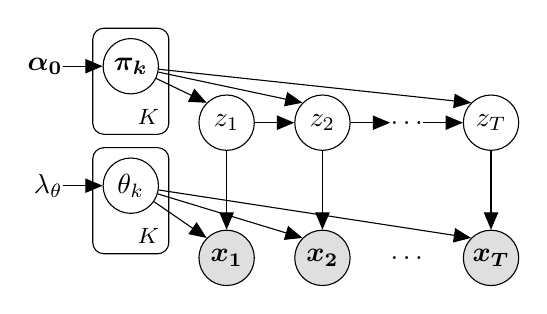
\begin{tikzpicture}[x=0.5cm,y=0.5cm]

  \node[obs] (x_1){$\boldsymbol{x_1}$};
  \node[obs, right=of x_1] (x_2){$\boldsymbol{x_2}$};
  \node[const, right=of x_2] (x_dots){$\ldots$};
  \node[obs, right=of x_dots] (x_T){$\boldsymbol{x_{T}}$};

  \node[latent, above=1cm of x_1] (z_1){$z_1$};
  \node[latent, right=of z_1] (z_2){$z_2$};
  \node[const, right=of z_2] (z_dots){$\ldots$};
  \node[latent, right=of z_dots] (z_T){$z_{T}$};

  \node[latent, yshift=-0.8 cm, left=of z_1] (theta_k){$\theta_k$};
  \node[latent, above=0.8cm of theta_k] (pi_k){$\boldsymbol{\pi_k}$};

  \node[const, left=of pi_k] (alpha_0){$\boldsymbol{\alpha_0}$};
  \node[const, left=of theta_k] (lambda_theta){$\lambda_\theta$};

  \edge{alpha_0}{pi_k};
  \edge{lambda_theta}{theta_k};
  \edge{pi_k}{z_1.north west};
  \edge{pi_k}{z_2.north west};
  \edge{pi_k}{z_T.north west};
  \edge{z_1}{z_2};
  \edge{z_1}{x_1};
  \edge{z_2}{z_dots};
  \edge{z_2}{x_2};
  \edge{z_dots}{z_T};
  \edge{z_T}{x_T};
  \edge{theta_k}{x_1.north west};
  \edge{theta_k}{x_2.north west};
  \edge{theta_k}{x_T.north west};

  \plate{K1}{(theta_k)}{$K$};
  \plate{K2}{(pi_k)}{$K$};

\end{tikzpicture}

\end{document}
